% Include Preamble 
\documentclass[10pt,dvipsnames, aspectratio=169]{beamer}
\usetheme[progressbar=frametitle]{metropolis}
\usepackage[]{verbatim}\usepackage[]{}
\usepackage{booktabs}
\usepackage[scale=2]{ccicons}
\usepackage[misc]{ifsym}
\usepackage{wasysym}
\usepackage{listings}
\usepackage{xspace}
\usepackage{amsmath}
\usepackage{xcolor}
\usepackage{ragged2e}\justifying % for justify content % Customize 
\setlength{\parskip}{5pt} % vertical spacing between 2 paragraphs
\setbeamersize{text margin left=12mm, text margin right=12mm} 
\setbeamertemplate{frametitle}[default][left, leftskip=8mm]
%\usepackage[hidelink]{hyperref}
\newcommand{\themename}{\textbf{\textsc{metropolis}}\xspace}

% WARNING: Don't Touch,if you are not compfortable! 
\addtobeamertemplate{frametitle}{}{
%\begin{tikzpicture}[remember picture,overlay]
%\node[anchor=north east,yshift=2pt,xshift=-65pt] at (current page.north east) 
%{\includegraphics[height=.75cm]{img/elixir-portugal-white}};
%\node[anchor=north east,yshift=4pt] at (current page.north east) 
%{
\includegraphics[height=1cm]{img/hdro}};
%\end{tikzpicture}
}

% Title Page of Presentation 
% WARNING: Don't change logo, just write your details 
\title{ISCB20.01 - Introduction to LINUX for Biologists}
\date{\today}
\author{Md. Jubayer Hossain\\
        https://jhossain.me/}
\institute{Lead Organizer, Introduction to Scientific Computing for Biologists 
\\ Founder, Health Data Research Organization}
\titlegraphic{\vspace{4cm}\hfill
\includegraphics[height=1cm]{img/hdro2}}

\begin{document}
\maketitle
% Section Title 
\section{Section--1.2: Working Environment Setup}
% Slide-1 
\begin{frame}[t]{Ubuntu Interface Introduction}
    \begin{itemize}
      \item Interface Tour 
      \item Basic Customization 
      \item Software Center 
    \end{itemize}
\end{frame}

% Slide-2 
\begin{frame}[t]{Terminal}
	\centering
	\begin{figure}[!h]
		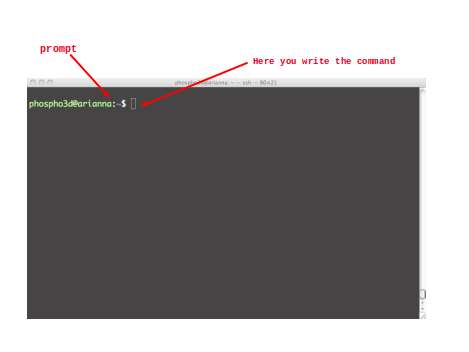
\includegraphics[scale=.7]{img/shell.png}
	\end{figure}
\end{frame}

% Slide-3
\begin{frame}[t]{System Update and Upgrade}
	\begin{itemize}
		\item \textbf{Update:} sudo apt update 
		\item \textbf{Upgrade:} sudo apt upgrade 
		\item \textbf{Update and Upgrade:} sudo apt update \&\& sudo apt 
		upgrade 
		\item \textbf{Update and Upgrade:} sudo apt update \&\& sudo apt 
		upgrade -y
	\end{itemize}
\end{frame}

% Slide-4
\begin{frame}[t]{Install ZSH}
	\begin{itemize}
		\item Visit -- 
		\url{https://github.com/ohmyzsh/ohmyzsh/wiki/Installing-ZSH}
		\item \textbf{Installation Process } \\ 
		\begin{itemize}
			\item \textbf{Update System:} sudo apt update
			\item \textbf{Install ZSH:} sudo apt install zsh
			\item \textbf{Check Version:} zsh --version
			\item \textbf{Check Path:} whereis zsh
			\item \textbf{Set as Default:} sudo usermod -s /usr/bin/zsh 
			\$(whoami)
			\item \textbf{Set Theme:} nano ~/.zshrc $\rightarrow$ 
			ZSH\_THEME="agnoster"
			
			\item \textbf{Restart Your Computer:} sudo reboot 
			\item \textbf{Installing Powerline and Powerline Fonts for ZSH:} \\
			sudo apt install powerline fonts-powerline
		\end{itemize}
	\end{itemize}
\end{frame}

% Slide-5
\begin{frame}[t]{Install Terminator}
	Much of the behaviour of Terminator is based on GNOME Terminal, and we are 
	adding more features from that as time goes by, but we also want to extend 
	out in different directions with useful features for sysadmins and other 
	users. If you have any suggestions, please file wishlist bugs! 
	(https://gnometerminator.blogspot.com/p/introduction.html)
	\begin{itemize}
		\item \textbf{Update:} sudo apt update 
		\item \textbf{Update:} sudo apt terminator  
	\end{itemize}
\end{frame}


% Slide-6
\begin{frame}[t]{Install (.deb) Packages}
	\begin{itemize}
		\item Gdebi lets you to install any deb packages without opening the 
		Default software centre in Ubuntu.
		\item \textbf{Install gdebi:} sudo apt install gdebi
		\item \textbf{Software Installation Steps using GDebi  Package 
		Installer}
		\begin{itemize}
			\item \textbf{Step-1:}  Open with Other Application 
			\item \textbf{Step-2:}  Select $\rightarrow$ GDebi Package Installer
			\item \textbf{Step-:3}  Click $\rightarrow$ Install Package 
			\item \textbf{Step-:4}  Give Your Password 
			\item \textbf{Step-:5}  Close 
		\end{itemize}
	\end{itemize}
\end{frame}

% Slide-7
\begin{frame}[t]{Download and Install Google Chrome}
	\begin{itemize}
		\item \textbf{Download Chrome for Linux:} 
		\url{https://www.google.com/chrome/}
		\item \textbf{Install Chrome} 
		\begin{itemize}
			\item \textbf{Step-1:}  Open with Other Application 
			\item \textbf{Step-2:}  Select $\rightarrow$ GDebi Package Installer
			\item \textbf{Step-:3}  Click $\rightarrow$ Install Package 
			\item \textbf{Step-:4}  Give Your Password 
			\item \textbf{Step-:5}  Close 
		\end{itemize}
	\end{itemize}
\end{frame}

\begin{frame}[t]{Download and Install Slack}
	\begin{itemize}
		\item \textbf{Download Slack for Linux:} 
		\url{https://slack.com/intl/en-bd/downloads/linux}
		\item \textbf{Install Slack} 
		\begin{itemize}
			\item \textbf{Step-1:}  Open with Other Application 
			\item \textbf{Step-2:}  Select $\rightarrow$ GDebi Package Installer
			\item \textbf{Step-:3}  Click $\rightarrow$ Install Package 
			\item \textbf{Step-:4}  Give Your Password 
			\item \textbf{Step-:5}  Close 
		\end{itemize}
	\end{itemize}
\end{frame}


% Slide-8
\begin{frame}[t]{Download and Install Anaconda Python Distribution}
	\begin{itemize}
		\item 
		\textbf{Download--}\url{https://repo.anaconda.com/archive/Anaconda3-2020.11-Linux-x86_64.sh}
		\item \textbf{Installation:} sh Anaconda3-2020.11-linux-x86\_64.sh
		\item \textbf{Activate:} source ~/.zshrc
		\item \textbf{Launch Jupyter:} anaconda-navigator 
	\end{itemize}
\end{frame}

% Slide-8
\begin{frame}[t]{Install R}
	\begin{itemize}
		\item 
		\textbf{CRAN 
		Website--}\url{https://cran.r-project.org/bin/linux/ubuntu/README.html}
		\item \textbf{Installation:} sudo deb 
		https://cloud.r-project.org/bin/linux/ubuntu focal-cran40/
		
		\item \textbf{To install the complete R system} 
		\begin{itemize}
			\item sudo apt update
			\item sudo apt-get install r-base
			\item sudo apt-get install r-base-dev
		\end{itemize}
	\end{itemize}
\end{frame}


% Slide-9
\begin{frame}[t]{RStudio}
	\begin{itemize}
		\item 
		\textbf{Download--}\url{https://rstudio.com/products/rstudio/download/}
		\begin{itemize}
			\item \textbf{Step-1:}  Open with Other Application 
			\item \textbf{Step-2:}  Select $\rightarrow$ GDebi Package Installer
			\item \textbf{Step-:3}  Click $\rightarrow$ Install Package 
			\item \textbf{Step-:4}  Give Your Password 
			\item \textbf{Step-:5}  Close 
		\end{itemize}
	\end{itemize}
\end{frame}
% Slide-10
\begin{frame}[t]{Text Editor--VSCode}
		\begin{itemize}
		\item 
		\textbf{Download--}\url{https://code.visualstudio.com/download}
		\begin{itemize}
			\item \textbf{Step-1:}  Open with Other Application 
			\item \textbf{Step-2:}  Select $\rightarrow$ GDebi Package Installer
			\item \textbf{Step-:3}  Click $\rightarrow$ Install Package 
			\item \textbf{Step-:4}  Give Your Password 
			\item \textbf{Step-:5}  Close 
		\end{itemize}
	\end{itemize}
\end{frame}

% Slide-11
\begin{frame}[t]{Install \LaTeX}
	\begin{itemize}
		\item \textbf{Install:} sudo apt install texlive-latex-extra
		\item \textbf{Install Publishers:} sudo apt install 
		texlive-publishers
	\end{itemize}
\end{frame}


% Slide-11
\begin{frame}[t]{{\LaTeX} Editor--TeXStudio}
	\begin{itemize}
		\item \textbf{Step-1:} Open Ubuntu Software Center
		\item \textbf{Step-2:} Search TeXStudio
		\item \textbf{Step-3:} Click Install 
		\item \textbf{Step-4:} Give Your Password 
	\end{itemize}
\end{frame}


\begin{frame}[t]{Download and Install Mendeley}
	\begin{itemize}
		\item \textbf{Download Mendeley for Linux :} 
		\url{https://www.mendeley.com/download-desktop-new/}
		\item \textbf{Install Slack} 
		\begin{itemize}
			\item \textbf{Step-1:}  Open with Other Application 
			\item \textbf{Step-2:}  Select $\rightarrow$ GDebi Package Installer
			\item \textbf{Step-:3}  Click $\rightarrow$ Install Package 
			\item \textbf{Step-:4}  Give Your Password 
			\item \textbf{Step-:5}  Close 
		\end{itemize}
	\end{itemize}
\end{frame}



% Thank you slide 
\plain{Thank You\\ \ \\ \Huge{\smiley}}

\end{document}